\documentclass[a4paper, 12pt, oneside]{scrbook}
\usepackage[hyphens,spaces,obeyspaces]{url}
\usepackage[sorting = none, backend=bibtex]{biblatex}
\usepackage[english]{babel}
\usepackage[T1]{fontenc}
\usepackage[utf8]{inputenc}
\usepackage[hidelinks]{hyperref}
\usepackage{graphicx}
\usepackage{subcaption}
\usepackage{epstopdf}
\usepackage{lmodern}
\usepackage{float}
\usepackage{acronym}
\usepackage{booktabs}
\usepackage{caption}
\usepackage{csquotes}
\usepackage{enumitem}
\usepackage{fancyhdr}
\usepackage{url}
\usepackage{listings}
\usepackage[table]{xcolor}
\usepackage{wrapfig}
\usepackage{forest}
\usepackage{tabularx}
\usepackage{colortbl}
\usepackage{booktabs}
\usepackage[onehalfspacing]{setspace}
\usepackage{amsmath}
\usepackage{threeparttable}
\usepackage[english]{cleveref}
\usepackage{listings}
\renewcommand*{\headfont}{\normalfont}
\renewcommand*{\multicitedelim}{\addsemicolon\space}
\renewcommand*{\headrulewidth}{0pt}
\renewcommand*{\arraystretch}{1.5}
\setlength{\parskip}{1.5ex}
\makeatletter
% define new boolean conditional switch for whether
% the abstract is being typeset
\newif\ifabstract
% redefine `\chapter` so it only starts a new page if not typesetting
% the abstract; sets abstract conditional to false after doing so
\renewcommand\chapter{\ifabstract\relax\else%
	\if@openright\cleardoublepage\else\clearpage\fi%
	\fi
	\abstractfalse%
	\thispagestyle{plain}%
	\global\@topnum\z@
	\@afterindentfalse
	\secdef\@chapter\@schapter}

% command for putting the title and name above the abstract; switches
% abstact boolean to true for next `\chapter*` command...
\newcommand{\conclusion}{
	\if@openright\cleardoublepage\else\clearpage\fi
		\begin{center}
			\textbf{\larger{Summary}}\par
			\emph{Hier kommt nach der Fertigstellung der Arbeit noch eine Zusammenfassung der Arbeit mit ein oder mehreren Sätzen hin. Hier kommt nach der Fertigstellung der Arbeit noch eine Zusammenfassung der Arbeit mit ein oder mehreren Sätzen hin. Hier kommt nach der Fertigstellung der Arbeit noch eine Zusammenfassung der Arbeit mit ein oder mehreren Sätzen hin2. }\par
		\end{center}

	\abstracttrue}
\makeatother
\lstset
{
         basicstyle=\footnotesize\ttfamily,
         numbers=left,               	% Ort der Zeilennummern
         numberstyle=\tiny,          	% Stil der Zeilennummern
%         stepnumber=2,               	% Abstand zwischen den Zeilennummern
         numbersep=5pt,              	% Abstand der Nummern zum Text
         tabsize=2,                  	% Groesse von Tabs
         extendedchars=true,
         breaklines=true,            	% Zeilen werden Umgebrochen
         keywordstyle=\color{red},
            frame=b,
 %        keywordstyle=[1]\textbf,    	% Stil der Keywords
 %        keywordstyle=[2]\textbf,
 %        keywordstyle=[3]\textbf,
 %        keywordstyle=[4]\textbf, \sqrt{\sqrt{}}
         stringstyle=\color{white}\ttfamily,
         showspaces=false,
         showtabs=false,
         xleftmargin=27pt,
         framexleftmargin=27pt,
         framexrightmargin=5pt,
         framexbottommargin=4pt,
%         backgroundcolor=\color{lightgray},
         showstringspaces=false      	% Leerzeichen in Strings anzeigen ?
}
\addbibresource{bibliography.bib}

\begin{document}
	\frontmatter
	
\def\title{Titel-TODO}
\def\abgabe{xx.xx.2023}

\begin{titlepage}
	
	
	
	\vspace{5pt}
	
	\begin{center}
		
		\Large \textbf\title
		
		\vspace{50pt}
		
		\large Studienarbeit T3\_3101
		
		von 
		
		\large \textbf{Rico Kursidem} 
		
		\vspace{15pt}
		
		im
		
		\large Studiengang Angewandte Informatik
		
		an der Dualen Hochschule Baden-Württemberg Mosbach

        \vspace{10pt}

        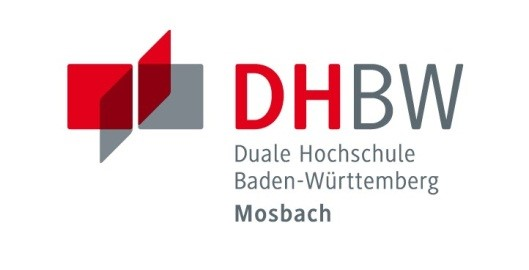
\includegraphics[height=3.5cm]{images/dhbw-logo.jpg}
		
		\vspace{20pt}
		
		\large Abgegeben am: \abgabe
		
		\vspace{30pt}

		
		\begin{table}[h]
			\centering
			\begin{tabular}{r l}
				\large\textbf{Matrikelnummer, Kurs} & \large 5451998, MOS-INF20B \\
                \large\textbf{Betreuer der Dualen Hochschule} & \large Philipp Abele \\
			\end{tabular}
			
		\end{table}
		
	\end{center}
	
	
\end{titlepage}
	\chapter*{Abbreviation} 
\begin{acronym}
	%A
	%B
	%C
	%D
	%E
	\acro{EDA}{Exploratory Data Analysis}
	%F
	%G
	%H
	%I
	\acro{IDA}{Initial Data Analysis}
	%J
	%K
	%L
	%M
	%N
	%O
	%P
	%Q
	%R
	%S
	%T
	%U
	%V
	%W
	%X
	%Y
	%Z
\end{acronym}
	\tableofcontents
	\listoffigures
	%\listoftables
	%\lstlistoflistings
	\nocite{*}

	\mainmatter

	\pagebreak
%	\conclusion
	\chapter{Introduction} 
	
	\chapter{Theoretical Basis}
	
		\section{Exploratory Data Analysis}
			
			\noindent Frederik Hardwig describes Exploratory Data Analysis (\ac{EDA}) as two thinks. As a Way of Thinking and a Method to work with data. 
			The Data Miner should always keep in mind, that you need to look for new Patterns that weren't expected, because they are the most interesting. It is important not trying to proof your own Thesis from before the Analyzing Process but to find new ones and always keep open to new findings. Also the Data Analyst should be skeptic towards Methods that compromise Data. If Data is summarized there will always be some loss of Information and the Hypothesis that will be based on these results will be not complete. To avoid this it is a good thing being skeptic towards compressed data. 
			As a Method, \ac{EDA} works with a lot of visualization to find patterns in Datasets. It is important not to confuse Data Analysis and Statistics. It is important to keep in mind that even the most used statistical Methods could have some hidden assumptions about the data. It is always suggested to use diagrams and other visual methods to display data to minimize errors resulting out of these assumptions.\cite{Hardwig:Explortory_Data_Analysis}
			
			\noindent \ac{EDA} tries to be find new Hypothesis in the data and not to proof already stated ones. This contrasts the Initial Data Analysis (\ac{IDA}) where it is more conman to look closely for findings that are needed to develop a modal and hypothesis testing. The goals of \ac{EDA} is to develop and evaluate Hypothesis, provide recommendations for statistical Techniques to support the analyzing process and provide Methods to collect more Data. 
			
			\noindent We can explore the most used graphical Methods on a sample dataset.
			
			%TODO: get Pictures into the documentation of EDA -> use iris exsample from Data mining cours
			
			 
	
	\chapter{Application}
	
	
	\chapter{Implementation}
	
	
	\chapter{Summary} % Fazit
	
	\frontmatter
	\printbibliography
\end{document}
